\documentclass[xcolor=pdflatex,dvipsnames,table]{beamer}
\usepackage{epsfig,graphicx}
\usepackage{palatino}
\usepackage{fancybox}
\usepackage{relsize}
\usepackage[procnames]{listings}
\usepackage{hyperref}
\usepackage{qtree}
\usepackage{booktabs}



% fatter TT font
\renewcommand*\ttdefault{txtt}
% another TT, suggested by Alex
% \usepackage{inconsolata}
% \usepackage[T1]{fontenc} % needed as well?

\usepackage[procnames]{listings}

\newcommand{\scale}{0.7}

\newif\ifbook
% shared in slides and book

\lstdefinelanguage{chisel}{
  morekeywords={abstract,case,catch,class,def,%
    do,else,extends,false,final,finally,%
    for,if,implicit,import,match,mixin,%
    new,null,object,override,package,%
    private,protected,requires,return,sealed,%
    super,this,throw,trait,true,try,%
    type,val,var,while,with,yield},
  otherkeywords={=>,<-,<\%,<:,>:,\#,@},
  sensitive=true,
  morecomment=[l]{//},
  morecomment=[n]{/*}{*/},
  morestring=[b]",
  morestring=[b]',
  morestring=[b]"""
}

\usepackage{color}
\definecolor{dkgreen}{rgb}{0,0.6,0}
\definecolor{gray}{rgb}{0.5,0.5,0.5}
\definecolor{mauve}{rgb}{0.58,0,0.82}

% Default settings for code listings
\ifbook
\lstset{%frame=lines,
  language=chisel,
  aboveskip=3mm,
  belowskip=3mm,
  showstringspaces=false,
  columns=fixed, % basewidth=\mybasewidth,
  basicstyle={\small\ttfamily},
  numbers=none,
  numberstyle=\footnotesize,
  % identifierstyle=\color{red},
  breaklines=true,
  breakatwhitespace=true,
  procnamekeys={def, val, var, class, trait, object, extends},
  % procnamestyle=\ttfamily,
  tabsize=2,
  float
}
\else
\lstset{%frame=lines,
  language=chisel,
  aboveskip=3mm,
  belowskip=3mm,
  showstringspaces=false,
  columns=fixed, % basewidth=\mybasewidth,
  basicstyle={\small\ttfamily},
  numbers=none,
  numberstyle=\footnotesize\color{gray},
  % identifierstyle=\color{red},
  keywordstyle=\color{blue},
  commentstyle=\color{dkgreen},
  stringstyle=\color{mauve},
  breaklines=true,
  breakatwhitespace=true,
  procnamekeys={def, val, var, class, trait, object, extends},
  procnamestyle=\ttfamily\color{red},
  tabsize=2,
  float
}
\fi

\lstnewenvironment{chisel}[1][]
{\lstset{language=chisel,#1}}
{}

\newcommand{\shortlist}[1]{{\lstinputlisting[nolol]{#1}}}

\newcommand{\longlist}[3]{{\lstinputlisting[float, caption={#2}, label={#3}, frame=tb, captionpos=b]{#1}}}

\newcommand{\verylonglist}[3]{{\lstinputlisting[caption={#2}, label={#3}, frame=tb, captionpos=b]{#1}}}


\hypersetup{
  linkcolor  = black,
%  citecolor  = blue,
  urlcolor   = blue,
  colorlinks = true,
}

\newcommand{\code}[1]{{\texttt{#1}}}

\beamertemplatenavigationsymbolsempty
\setbeamertemplate{footline}[frame number]

\newcommand{\todo}[1]{{\emph{TODO: #1}}}
\newcommand{\martin}[1]{{\color{blue} Martin: #1}}
\newcommand{\abcdef}[1]{{\color{red} Author2: #1}}

% uncomment following for final submission
%\renewcommand{\todo}[1]{}
%\renewcommand{\martin}[1]{}
%\renewcommand{\author2}[1]{}


\title{Digital Electronics 2: Introduction}
\author{Martin Schoeberl}
\date{\today}
\institute{Technical University of Denmark\\
Embedded Systems Engineering}

\begin{document}

\begin{frame}
\titlepage
\end{frame}


\begin{frame}[fragile]{Overview}
\begin{itemize}
\item Motivation and the digital abstraction
\item Course organization
\item Languages for hardware design
%\item Testing (see 2.1.4)
\item A first round in Chisel
\item Tools and tool setup
\end{itemize}
\end{frame}


\begin{frame}[fragile]{A BIG Chip}
\begin{itemize}
\item \url{https://singularityhub.com/2019/08/26/this-giant-ai-chip-is-the-size-of-an-ipad-and-holds-1-2-trillion-transistors/}
\item $1.2 \times 10^{12}$ transistors
\item If you design 1 gate (= 4 transistors) per second
\begin{itemize}
\item It takes you 10 thousand years!
\end{itemize}
\item This calls for some abstraction
\end{itemize}
\end{frame}

\begin{frame}[fragile]{Digital Systems are Everywhere}
\begin{itemize}
\item Digital systems are all over in our live
\item No more analog media
\item CD, mobile phone, TV, DVD,... all digital now
\item Analog circuits only at the edge
\item The rest is processed in digital
\item If performance allows, functions are moved to software
\item But processor speedup has slowed down
\item Algorithms are moved back into hardware
\end{itemize}
\end{frame}

\begin{frame}[fragile]{FPGAs in the Cloud}
\begin{itemize}
\item High performance algorithm in an FPGA
\item \href{https://aws.amazon.com/ec2/instance-types/f1/}{An FPGA in the cloud}
\item \href{https://www.intel.com/content/www/us/en/products/docs/storage/programmable/applications/cloud.html}{Intel offers FPGAs for servers}
\begin{itemize}
\item There is some reason why Intel bought Altera
\end{itemize}
\item We need digital designers to make this work
\item A good time to be a digital designer
\end{itemize}
\end{frame}

\begin{frame}[fragile]{The Digital Abstraction}
\begin{columns}
 
\column{0.5\textwidth}
\begin{itemize}
\item Just two values: 0 and 1, or low and hight
\item Represented as voltage
\item Digital signals tolerate noise
\item Digital Systems are \emph{simple}, just:
\begin{itemize}
\item Combinational circuits and
\item Registers
\end{itemize}
\end{itemize}
 
\column{0.5\textwidth}
\begin{figure}
  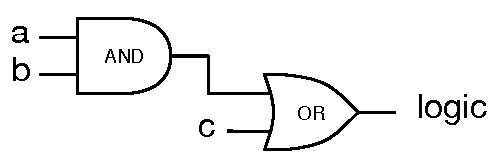
\includegraphics[scale=\scale]{../figures/logic}
\end{figure}
\begin{figure}
  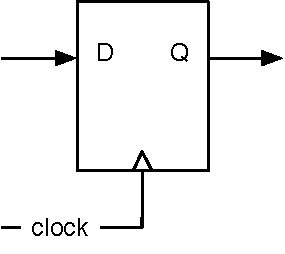
\includegraphics[scale=\scale]{../figures/register}
\end{figure}
\end{columns}

\end{frame}

\begin{frame}[fragile]{Hardware Design in DK}
\begin{itemize}
\item Demant (former Oticon)
\item Widex
\item GN ReSound
\item Microsemi
\item Intel (former Altera) Denmark
\item probably some more...
\item 
\item They are all hiring
\end{itemize}
\end{frame}

\begin{frame}[fragile]{Example Design from Microsemi DK}
A picture of the board with the \$50k Xilinx FPGA. This is a new board and is developed for ASIC prototyping in order to do pre-silicon validation as well as SW development. We have on the board currently mapped our current project: 8port industrial gigabit Ethernet switch with full TSN, CPU system ARM A7 with DDR, USB, PCIe and hardware security engines (SHA, AES) for secure boot of Linux and on the fly DRAM encryption. We scale and map all the digital logic to the FPGA.
\begin{itemize}
\item Show the picture
\end{itemize}
\end{frame}

\begin{frame}[fragile]{Digital Design within an EE Master}
\begin{itemize}
\item Not an obvious choice, as there is no specialization in digital systems
\item Select some of the following courses
\begin{itemize}
\item 02155: Computer Architecture and Engineering
\item 02203: Design of Digital Systems
\item 02211: Advanced Computer Architecture
\item 02205: VLSI Design
\item 02217: Design of Arithmetic Processors
\item 02204: Design of Asynchronous Circuits
\item 02209: Test of Digital Systems
\end{itemize}
\end{itemize}
\end{frame}

\begin{frame}[fragile]{Computer Engineering Education at DTU}
\begin{itemize}
\item On the border between hardware and software
\item Very well payed jobs :-)
\item Not an easy choice at DTU as well
\begin{itemize}
\item No BSc available
\item Between EE and CS
\end{itemize}
\item Start with Bsc. in EE
\item Specialization in Indlejrede systemer og programmering
\begin{itemize}
\item 02155: Computer Architecture and Engineering
\item 02105: Algoritmer og datastrukturer
\end{itemize}
\item Continue as MSc. in Computer Science and Engineering
\item Specialization in
\begin{itemize}
\item Digital Systems
\item Embedded and Distributed Systems
\end{itemize}
\end{itemize}
\end{frame}

\begin{frame}[fragile]{Web Resources}
\begin{itemize}
\item \href{https://cn.inside.dtu.dk/cnnet/element/612883/frontpage}{DTU Inside}
\begin{itemize}
\item Vending machine document
\item Project report hand in
\end{itemize}
\item \href{http://www2.imm.dtu.dk/courses/02139/}{Course website}
\begin{itemize}
\item General information, starting point
\end{itemize}
\item \href{https://github.com/schoeberl/chisel-lab}{Lab website}
\begin{itemize}
\item Lab material on GitHub
\end{itemize}
\item \href{http://www.imm.dtu.dk/~masca/chisel-book.html}{Chisel book website}
\begin{itemize}
\item Download the free PDF
\end{itemize}
\end{itemize}
\end{frame}

\begin{frame}[fragile]{Organization and Workload}
\begin{itemize}
\item Usually 2 hours lectures and 2 hours supervised lab
\item 5 ECTS is equivalent to 9 hours per week
\item That means 5 hours work on your own
\begin{itemize}
\item Do some reading, prepare for the lecture and lab
\item Get the tools installed on your laptop
\item You have an FPGA board, experiment with it
\end{itemize}
\item You will learn a lot in this course, it will make you a better:
\begin{itemize}
\item engineer
\item hardware designer
\item programmer, and
\item computer user in general
\end{itemize}
\item Try to have fun with building stuff that is real!
\end{itemize}
\end{frame}

\begin{frame}[fragile]{Communication and Getting Help}
\begin{itemize}
\item Several sources of information:
\begin{itemize}
\item The Internet, Google, and Stackoverflow
\item Your fellow students (e.g., via Slack)
\item The TAs: \href{https://cn.inside.dtu.dk/cnnet/element/612883/participants}{Simon, Kasper, and Anthon}
\item Me
\end{itemize}
\item We will use Slack for easy communication (if ok for you)
\begin{itemize}
\item \url{https://de2019.slack.com/}
\end{itemize}
\item You can always just knock my door or shoot me an email
\item Anonymous feedback
\end{itemize}
\end{frame}

\begin{frame}[fragile]{Anonymous Feedback}
\begin{itemize}
\item Inbox available at: 
\href{https://docs.google.com/forms/d/e/1FAIpQLSclKyEM_foF7U0TF-CoIZhla5EFEcE8-EGD7Jvle6TBB90WZw/viewform?vc=0&c=0&w=1&usp=mail_form_link}{Anonymous Inbox}
\item Simple Google form without revealing your identity
\item I will get notified by an email
\item Use when you want to complain, give feedback, but also when you like something ;-)
\item Even when frustrated, please be polite, a human is reading this
\end{itemize}
\end{frame}

\begin{frame}[fragile]{Cheating and Plagiarism}
\begin{itemize}
\item It is ok and good practice to discuss problems and solutions with your fellow students
\item But you need to hand in your own solution
\item Copying stuff or offering stuff for copying is cheating
\item Copying material from somewhere is plagiarism and copyright violation
\item Cheating is handled quite rigorous at DTU, you might get expelled
\item Using source code control (GitHub) is good practice
\item However, keep it private. Otherwise you might contribute to cheating
\end{itemize}
\end{frame}


\begin{frame}[fragile]{This is an Open-Access/Open-Source Course}
\begin{itemize}
\item Almost all material is public visible
\item Slides are open access
\item Lab material is open access
\item Hosted on GitHub
\begin{itemize}
\item \textbf{You} can contribute with a pull request
\item Becoming an author of this course :-)
\end{itemize}
\item The Chisel book is freely available
\end{itemize}
\end{frame}

\begin{frame}[fragile]{Lab Work}
\begin{itemize}
\item Some paper and pencil exercises
\item Most work on designing digital circuits with a hardware description language
\item Builds up to the final project: a vending machine
\item The vending machine and the report are graded
\end{itemize}
\end{frame}

\begin{frame}[fragile]{A Vending Machine from 1952}
\begin{figure}
    \centering
    \href{https://en.wikipedia.org/wiki/File:CandiesVendingMachine1952.jpg}{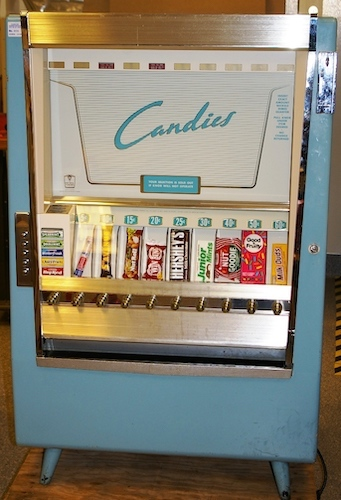
\includegraphics[scale=0.4]{CandiesVendingMachine1952}}

\end{figure}

{\tiny Source: Minnesota Historical Society, \href{https://creativecommons.org/licenses/by-sa/2.0}{CC BY-SA 2.0}}
\end{frame}

\begin{frame}[fragile]{The Vending Machine}
\begin{itemize}
\item Final project is a vending machine
\item Inputs: coins, buy
\item Display: price and current ammount
\item Output: release can or error
\item Small challenge to multiplex the display
\item State machine with data path is the \emph{brain} of the VM
\item Will be guided step by step over several weeks
\item More details next week
\item VM in hardware versus VM in software
\begin{itemize}
\item This is an exercise that you can solve with reasonable effort
\end{itemize}
\end{itemize}
\end{frame}


\begin{frame}[fragile]{Motivating Example for Chisel:\\
Lipsi: Probably the Smallest Processor in the World}
\begin{itemize}
\item Tiny processor
\item Simple instruction set
\item Shall be small
\begin{itemize}
\item Around 200 logic cells, one FPGA memory block
\end{itemize}
\item Hardware described in Chisel
\item Available at \url{https://github.com/schoeberl/lipsi}
\item Usage
\begin{itemize}
\item Utility processor for small stuff
\item Could be used for your vending machine
\item In teaching for introduction to computer architecture
\end{itemize}
\item The design took place on the island Lipsi
\end{itemize}
\end{frame}

\begin{frame}[fragile]{The Design of Lipsi on Lipsi}
\begin{figure}
    \centering
    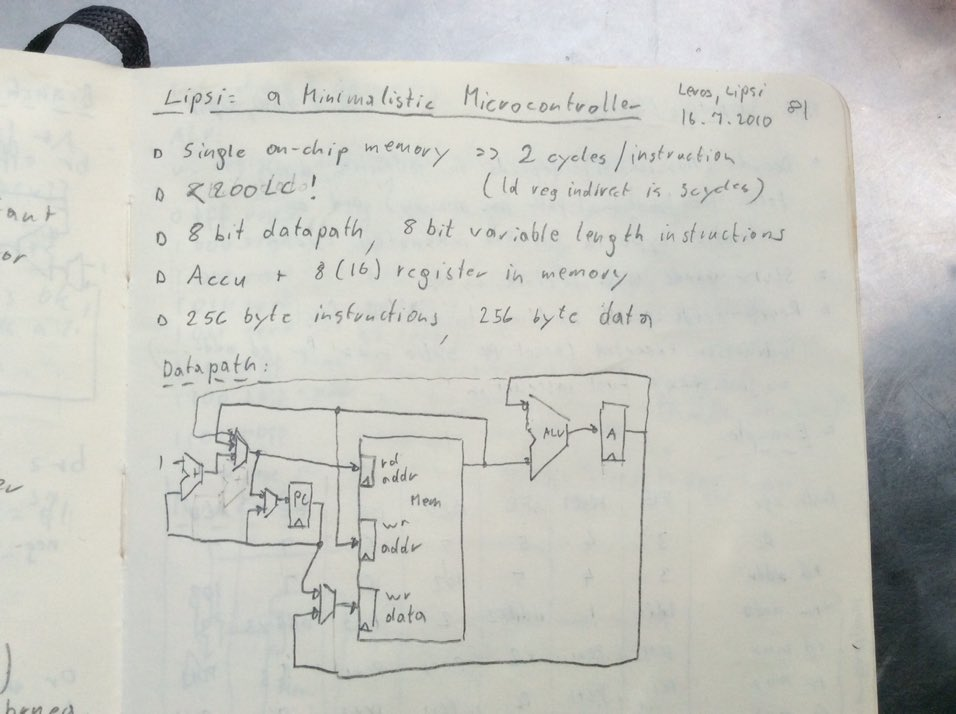
\includegraphics[scale=0.3]{../slides-tutorial/lipsi}
\end{figure}
\end{frame}

\begin{frame}[fragile]{Lipsi Implementation}
\begin{itemize}
\item Hardware described in Chisel
\item Tester in Chisel
\item Assembler in Scala
\begin{itemize}
\item Core case statement about 20 lines
\end{itemize}
\item Reference design of Lipsi as software simulator in Scala
\item Testing:
\begin{itemize}
\item Self testing assembler programs
\item Comparing hardware with a software simulator
\end{itemize}
\item All in a single programming language!
\item All in a single program
\item How much work is this?
\end{itemize}
\end{frame}

\begin{frame}[fragile]{Chisel is Productive}
\begin{itemize}
\item All coded and tested in less than 14 hours!
\end{itemize}
\begin{itemize}
\item The hardware in Chisel
\item Assembler in Scala
\item Some assembler programs (blinking LED)
\item Simulation in Scala
\item Two testers
\end{itemize}
\begin{itemize}
\item BUT, this does not include the design (done on paper)
\end{itemize}
\end{frame}

\begin{frame}[fragile]{Motivating Example: Lipsi, a Tiny Processor}
\begin{itemize}
\item Show in IntelliJ (if beamer allows)
\end{itemize}
\end{frame}

\begin{frame}[fragile]{The Slides are Online}
\begin{itemize}
\item \url{http://www2.imm.dtu.dk/courses/02139/}
\item \url{https://github.com/schoeberl/chisel-book/tree/master/slides}
\end{itemize}
%\begin{figure}
%    \centering
%    
\includegraphics[scale=0.5]{slides-link}
%\end{figure}
\end{frame}

\begin{frame}[fragile]{Why Chisel Instead of VHDL/Verilog/SystemVerilog?}
\begin{itemize}
\item Company O does Verilog, company W does VHDL
\begin{itemize}
\item Why Chisel?
\end{itemize}
\item We learn principles of digital design, not tools
\begin{itemize}
\item We pick a language that is modern and productive
\end{itemize}
\item When knowing principles, switching the language is a matter of a week
\item You are the future engineers and shall learn new tools
\item You may then bring Chisel into the company
\end{itemize}
\end{frame}

\begin{frame}[fragile]{More on Chisel Success Stories}
\begin{itemize}
\item Last week at CCC 2020 in silicon valley
\item 90 participants
\item More than 30 different chip companies present
\item Several companies are looking into Chisel
\item IBM did an open-source PowerPC
\item \href{https://www.sifive.com/}{SiFive} is a RISC-V startup success
\begin{itemize}
\item High productivity with Chisel
\item Open-source Rocket chip
\end{itemize}
\item Esperanto uses the BOOM processor in Chisel
\item Google did a machine learning processor
\item Intel is looking at Chisel
\item Chisel is open-source, if there is a bug you can fix it
\begin{itemize}
\item You can even contribute to the Chisel ecosystem :-)
\end{itemize}
\end{itemize}
\end{frame}

\begin{frame}[fragile]{Introduction to Chisel}
\begin{itemize}
\item Get an idea what Chisel is
\begin{itemize}
\item Will show you code snippets
\end{itemize}
\item Basic hardware constructs in Chisel
\item Pointers to more information
\item Have your first Chisel design running in an FPGA!
\begin{itemize}
\item From 0 to 100 in one afternoon
\end{itemize}\end{itemize}
\end{frame}


\begin{frame}[fragile]{Chisel}
\begin{itemize}
\item A hardware \emph{construction} language
\begin{itemize}
\item Constructing Hardware In a Scala Embedded Language
\item If it compiles, it is synthesisable hardware 
\item Say goodby to your unintended latches
\end{itemize}
\item Chisel is not a high-level synthesis language
\item Single source for two targets
\begin{itemize}
\item Cycle accurate simulation (testing)
\item Verilog for synthesis
\end{itemize}
\item Embedded in Scala
\begin{itemize}
\item Full power of Scala available
\item But to start with, no Scala knowledge needed
\end{itemize}
\item Developed at UC Berkeley
\end{itemize}
\end{frame}

\begin{frame}[fragile]{The C Language Family}

\Tree[.C [
   [.{\bf Verilog} {\bf SystemVerilog} ]
   [.C++  \emph{SystemC}  ]
   [.Java [.Scala {\bf Chisel} ] ]
   [.C\# ] ] ]
 
\end{frame}

\begin{frame}[fragile]{Other Language Families}

\begin{columns}
\column{0.5\textwidth}
\begin{center}
\Tree[.{Algol 68} [.Ada [.{\bf VHDL} ] ] ]
\end{center}
\column{0.5\textwidth}
\begin{center}
\Tree[.Python [.{\bf MyHDL} ] ]
\end{center}
\end{columns}
\end{frame}

\begin{frame}[fragile]{Some Notes on Scala}
\begin{itemize}
\item Object oriented
\item Functional
\item Strongly typed
\begin{itemize}
\item With very good type inference
\end{itemize}
\item Could be seen as Java++
\item Compiled to the JVM
\item Good Java interoperability
\begin{itemize}
\item Many libraries available
\item You can write your testing code in Java
\end{itemize}
\end{itemize}
\end{frame}

\begin{frame}[fragile]{Chisel vs. Scala}
\begin{itemize}
\item A Chisel hardware description is a Scala program
\item Chisel is a Scala library
\item When the program is executed it generates hardware
\item Chisel is a so-called \emph{embedded domain-specific language}
\end{itemize}
\end{frame}

\begin{frame}[fragile]{A Small Language}
\begin{itemize}
\item Chisel is a \emph{small} language
\item On purpose
\item Not many constructs to remember
\item The \href{https://github.com/freechipsproject/chisel-cheatsheet/releases/latest/download/chisel_cheatsheet.pdf}{Chisel Cheatsheet} fits on two pages
\item The power comes with Scala for circuit generators
\item With Scala, Chisel can grow with you
\end{itemize}
\end{frame}

\begin{frame}[fragile]{Tool Flow for Chisel Defined Hardware}
\begin{figure}
    \centering
    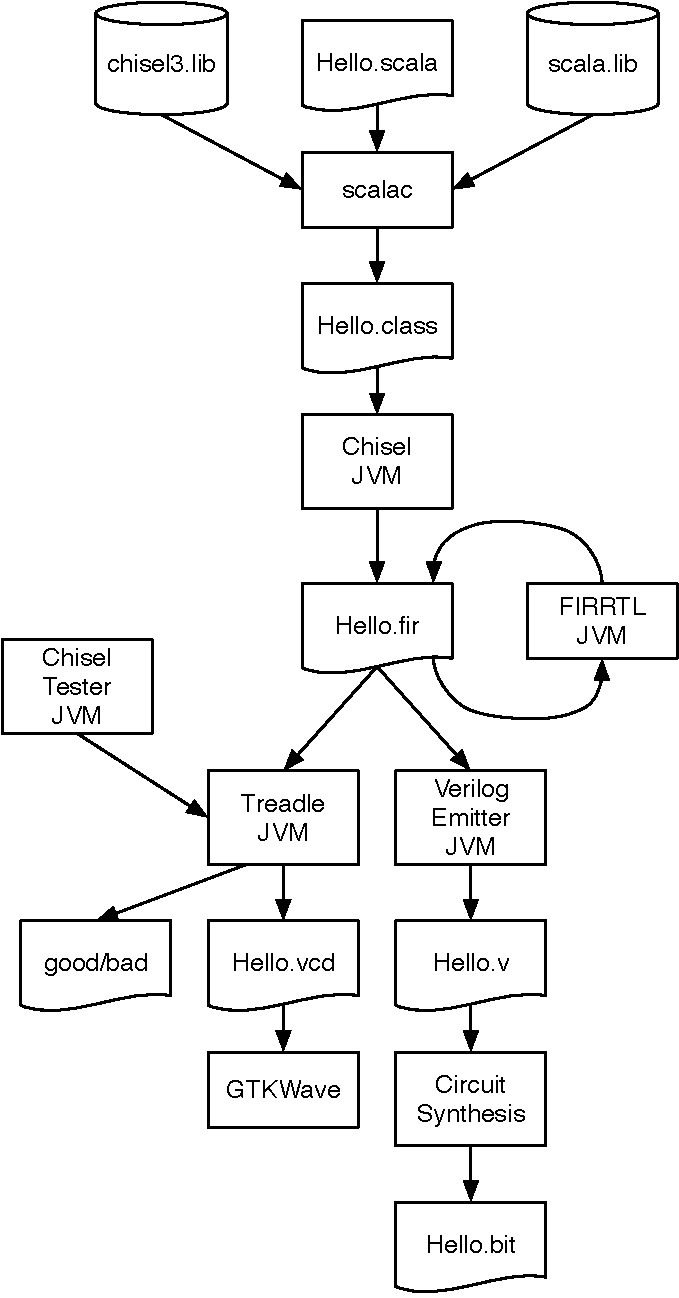
\includegraphics[scale=0.35]{../figures/flow}
\end{figure}
\end{frame}

\begin{frame}[fragile]{Signal Types}
\begin{itemize}
\item All types in hardware are a collection of bits
\item The base type in Chisel is \code{Bits}
\item \code{UInt} represents an unsigned integer
\item \code{SInt} represents a signed integer (in two's complement)
\end{itemize}
\shortlist{../code/types.txt}
\end{frame}

\begin{frame}[fragile]{Number of Bits: n.W}
\begin{itemize}
\item A collection of bits has a \emph{width}
\item The width is the number of bits
\item Is written as number followed by \code{.W}
\item Following example shows the width of \code{n}
\end{itemize}
\shortlist{../code/n_w.txt}
\end{frame}

\begin{frame}[fragile]{Constants}
\begin{itemize}
\item Constants can represent signed or unsigned numbers
\item We use \code{.U} and \code{.S} to distinguish
\end{itemize}
\shortlist{../code/constants.txt}
\begin{itemize}
\item Constants can also be specified with a width
\end{itemize}
\shortlist{../code/const_width.txt}
\end{frame}

\begin{frame}[fragile]{Hexadecimal and Binary Representation}
\begin{itemize}
\item We can specify constants with a different base
\item May come handy sometimes
\end{itemize}
\shortlist{../code/const_base.txt}
\end{frame}

\begin{frame}[fragile]{Boolean Values}
\begin{itemize}
\item Type for logical values
\item Can be \code{true} or \code{false}
\item Almost exchangeable with \code{UInt(1.W)}
\item Sometimes a signal, such as \code{valid}, may be better represented by a Boolean type
\end{itemize}
\shortlist{../code/bool.txt}
\end{frame}

\begin{frame}[fragile]{Combinational Circuits}
\begin{itemize}
\item Chisel uses Boolean operators, similar to C or Java
\item \code{\&} is the AND operator and \code{|} is the OR operator
\item The following code is the same as the schematics
\item \code{val logic} gives the circuit/expression the name \code{logic}
\item That name can be used in following expressions
\end{itemize}
\begin{figure}
  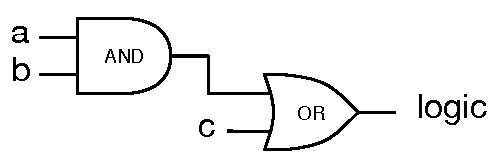
\includegraphics[scale=\scale]{../figures/logic}
\end{figure}
\shortlist{../code/logic.txt}
\end{frame}

\begin{frame}[fragile]{Standard Logic Operations}
\shortlist{../code/bool_ops.txt}
\begin{itemize}
\item Note that we do not need to define the width of the values
\item Note also that this is \emph{hardware}
\item All expressions are evaluated in parallel
\item Order does not matter
\end{itemize}
\end{frame}

\begin{frame}[fragile]{Arithmetic Operations}
\begin{itemize}
\item Same as in Java or C
\item The width of the result is automatically computed
\item E.g., the width of the multiplication is the sum of the width of \code{a} and the width of \code{b} 
\end{itemize}
\shortlist{../code/arith_ops.txt}
\end{frame}

\begin{frame}[fragile]{Wires}
\begin{itemize}
\item A signal (or wire) can be first defined
\item And later assigned an expression with \code{:=}
\end{itemize}
\shortlist{../code/wire.txt}
\end{frame}

\begin{frame}[fragile]{Chisel Defined Hardware Operators}
\begin{table}
{\footnotesize
  \begin{tabular}{lll}
    \toprule
    Operator & Description & Data types \\
    \midrule
    \code{* / \%} & multiplication, division, modulus & UInt, SInt \\
    \code{+ -} & addition, subtraction & UInt, SInt \\
    \code{=== =/=} & equal, not equal & UInt, SInt, returns Bool \\
    \code{> >= < <=} & comparison & UInt, SInt, returns Bool \\
    \code{<< >>} & shift left, shift right (sign extend on SInt) & UInt, SInt \\
    \code{\~} & NOT & UInt, SInt, Bool \\
    \code{\& | \^} & AND, OR, XOR & UInt, SInt, Bool \\
    \code{!} & logical NOT & Bool \\
    \code{\&\& ||} & logical AND, OR & Bool \\
    \bottomrule 
  \end{tabular} 
  }
\end{table}
\end{frame}

\begin{frame}[fragile]{Subfields and Concatenation}
A single bit can be extracted as follows:
\shortlist{../code/single_bit.txt}

\noindent A subfield can be extracted from end to start position:
\shortlist{../code/sub_field.txt}

\noindent Bit fields are concatenated with \code{Cat}:
\shortlist{../code/concat.txt}
\end{frame}


\begin{frame}[fragile]{A Multiplexer}
\begin{figure}
  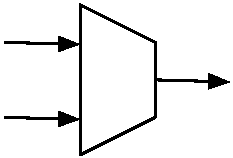
\includegraphics[scale=\scale]{../figures/mux}
\end{figure}
\begin{itemize}
\item A Multiplexer selects between alternatives
\item So common that Chisel provides a construct for it
\item Selects \code{a} when \code{sel} is \code{true.B} otherwise \code{b}
\end{itemize}
\shortlist{../code/mux.txt}
\end{frame}

\begin{frame}[fragile]{Conditional Update}
\begin{itemize}
\item With \code{when} we can express a conditional update
\item The resulting circuit is a multiplexer
\item In contrast to the \code{Mux} component, we can have several assignments in the \code{when} block
\item The rule is the the last enabled assignment counts
\begin{itemize}
\item Here the order of statements has a meaning
\end{itemize}
\end{itemize}
\shortlist{../code/comb_wire.txt}
\end{frame}

\begin{frame}[fragile]{The World of Combinational Logic}
\begin{itemize}
\item With the shown operations (logic, arithmetic, Mux) all possible combinational circuits can be described
\item Even the \code{Mux} is already \emph{syntactic sugar}
\begin{itemize}
\item A \code{Mux} is basically: \code{(a \& sel) | (b \& !sel)}
\end{itemize}
\item But Chisel provides further constructs for more elegant description of circuits
\item Stay tuned!
\end{itemize}
\end{frame}


\begin{frame}[fragile]{Register}
\begin{itemize}
\item A register is a collection of flip-flops
\item Updated on the rising edge of the clock
\item May be set to a value on reset
\item Clock and reset are implicitly connected to the register
\item A register can be any Chisel type that can be represented as a collection of bits
\end{itemize}

\end{frame}

\begin{frame}[fragile]{A Register with Reset}

\begin{figure}
  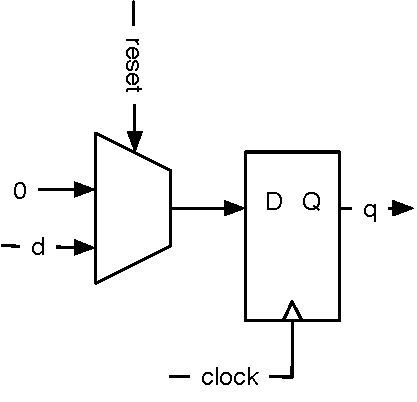
\includegraphics[scale=\scale]{../figures/register-reset-0}
\end{figure}
\end{frame}

\begin{frame}[fragile]{A Register with Reset}

Following code defines an 8-bit register, initialized with 0 at reset:

\shortlist{../code/register.txt}

\noindent An input is connected to the register with the \code{:=} update operator and
the output of the register can be used just with the name in an expression:

\shortlist{../code/reg_con.txt}
\end{frame}


\begin{frame}[fragile]{Hello World in Chisel}
\shortlist{../code/hello.txt}
\end{frame}

\begin{frame}[fragile]{Chisel is a Hardware Construction Language}
\begin{itemize}
\item The code I showed you looks much like Java code
\item But it is \emph{not} a program in the usual sense
\item It represents a circuit
\item The ``program'' constructs the circuit
\item All statements are ``executed'' in parallel
\item Statement order has mostly no meaning
\end{itemize}
\end{frame}

\begin{frame}[fragile]{Free Tools for Chisel and FPGA Design}
\begin{itemize}
\item \href{https://adoptopenjdk.net/}{Java OpenJDK 8} already installed for Java course
\item \href{https://www.scala-sbt.org/}{sbt, the Scala (and Java) build tool}
\item \href{https://www.jetbrains.com/idea/download/}{IntelliJ (the free Community version)}
\item \href{http://gtkwave.sourceforge.net/}{GTKWave}
\item \href{https://www.xilinx.com/products/design-tools/vivado/vivado-webpack.html}{Vivado WebPACK} already installed from DE1
% \item \href{http://www.altera.com/products/software/quartus-ii/web-edition/qts-we-index.html}{Quartus}
\item Nice to have:
\begin{itemize}
\item make, git
\end{itemize}
\end{itemize}
\end{frame}

\begin{frame}[fragile]{Tool Setup for Different OSs}
\begin{itemize}
\item Windows
\begin{itemize}
\item Use the installers from the websites
\end{itemize}
\item macOS
\begin{itemize}
\item \code{brew install sbt}
\item For the rest, use the installer from the websites
\item Use an Ubuntu VM to run Vivado
\end{itemize}
\item Linux/Ubuntu
\begin{itemize}
\item \code{sudo apt install openjdk-8-jdk git make gtkwave}
\item Install sbt, see \url{https://github.com/schoeberl/chisel-lab/blob/master/Setup.md}
\item IntelliJ as from the website
\end{itemize}
\item If setup fails, we have you covered with the databar PCs
\end{itemize}
\end{frame}

\begin{frame}[fragile]{Virtual Machine Setup for Chisel}
\begin{itemize}
\item Ubuntu based
\item \href{http://patmos.compute.dtu.dk/patmos-dev.zip}{Ubuntu VM with Quartus} uid: patmos, pwd: patmos
\item \href{https://patmos-download.compute.dtu.dk/de2lab.zip}{Ubuntu VM with Vivado} uid: de2lab, pwd: de2lab
\begin{itemize}
\item But this is VERY large (40 GB for the .zip file)
\end{itemize}
\item Use the  \href{https://www.vmware.com/products/workstation-player.html} {VMWare Workstation Player} (free for Linux and Windows)
\end{itemize}
\end{frame}

\begin{frame}[fragile]{An IDE for Chisel}
\begin{itemize}
\item IntelliJ
\item Scala plugin
\item For IntelliJ: File - New - Project from Existing Sources..., open build.sbt
%\item But you are not compiling with Eclipse\\ and against the Chisel source
\item Show it (down to the Basys3)
\end{itemize}
\end{frame}


\begin{frame}[fragile]{A Chisel Book}
\begin{figure}
    \centering
    \href{https://github.com/schoeberl/chisel-book}{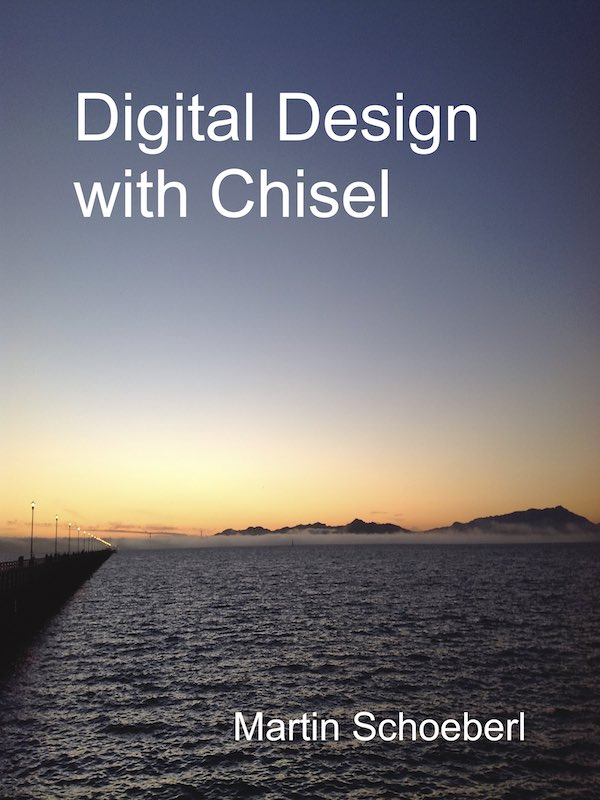
\includegraphics[scale=0.4]{../cover-small}}
\end{figure}

\begin{itemize}
\item Available in open access (as PDF)
\begin{itemize}
\item Optimized for reading on a tablet (size, hyper links)
\end{itemize}
\item Amazon can do the printout
\end{itemize}
\end{frame}

\begin{frame}[fragile]{Further Information}
\begin{itemize}
\item \url{https://www.chisel-lang.org/}
\item \url{https://github.com/freechipsproject/chisel-cheatsheet/releases/latest/download/chisel_cheatsheet.pdf}
\item \url{https://github.com/ucb-bar/chisel-tutorial}
\item \url{https://github.com/ucb-bar/generator-bootcamp}
%\item Chisel 2 documentation at \url{https://github.com/schoeberl/chisel2-doc}
%\begin{itemize}
%\item Chisel 2.2 Tutorial
%\item Getting Started with Chisel
%\end{itemize}
\item \url{http://groups.google.com/group/chisel-users}
\item \url{https://github.com/schoeberl/chisel-book}
\end{itemize}
\end{frame}


\begin{frame}[fragile]{Lab Time: Hello World in Chisel}
\begin{itemize}
\item Get a blinking LED working on your FPGA board
\item Clone or download the repository from:
\begin{itemize}
\item \url{https://github.com/schoeberl/chisel-lab}
\end{itemize}
\item Follow the instructions from the lab page
\begin{itemize}
\item Start IntelliJ and follow the instructions from the lab page
\item \code{sbt run}
\item Create a Vivado project
\item Synthesize with the Play button
\item Configure the FPGA with the Programmer button
\end{itemize}
\item {\bf You have your first Chisel design running in an FPGA!}
\end{itemize}
\end{frame}



\begin{frame}[fragile]{Change the Design}
\begin{itemize}
\item Use IntelliJ, \code{gedit}, or the editor you like most
\item Source is in \code{.../src/main/scala/Hello.scala}
\item Change blinking frequency
\item Rerun the example
\item Optional:
\begin{itemize}
\item Change to an asymmetric blinking, e.g., 200 ms on every second 
\end{itemize}
\end{itemize}
\end{frame}

\begin{frame}[fragile]{Summary}
\begin{itemize}
\item The world is digital
\item Processors do not get much faster -- we need to design custom hardware
\item We need a modern language for hardware/systems design for efficient/fast development
\item Chisel builds on the power of object-oriented and functional Scala
%\item Chisel is good for hardware generators
% \item You can get started with a hardware design in a special course or 4th semester project
\end{itemize}
\end{frame}

\end{document}

\begin{frame}[fragile]{Title}
\begin{itemize}
\item abc
\end{itemize}
\end{frame}
